\documentclass[letterpaper,10pt]{article}

\usepackage{titling}
\usepackage{listings}
\usepackage{url}
\usepackage{setspace}
\usepackage{subfig}
\usepackage{sectsty}
\usepackage{pdfpages}
\usepackage{colortbl}
\usepackage{multirow}
\usepackage{multicol}
\usepackage{relsize}
\usepackage{amsmath}
\usepackage{fancyvrb}
\usepackage{amsmath,amssymb,amsthm,graphicx,xspace}
\usepackage[titlenotnumbered,noend,noline]{algorithm2e}
\usepackage[compact]{titlesec}
\usepackage{XCharter}
\usepackage[T1]{fontenc}
\usepackage{tikz}
\usetikzlibrary{arrows,automata,shapes,trees,matrix,chains,scopes,positioning,calc}
\tikzstyle{block} = [rectangle, draw, fill=blue!20, 
    text width=2.5em, text centered, rounded corners, minimum height=2em]
\tikzstyle{bw} = [rectangle, draw, fill=blue!20, 
    text width=4em, text centered, rounded corners, minimum height=2em]

\newcommand{\CPP}{C\nolinebreak\hspace{-.05em}\raisebox{.4ex}{\tiny\bf +}\nolinebreak\hspace{-.10em}\raisebox{.4ex}{\tiny\bf +}}
\def\CPP{{C\nolinebreak[4]\hspace{-.05em}\raisebox{.4ex}{\tiny\bf ++}}}

\let\LaTeXtitle\title
\renewcommand{\title}[1]{\LaTeXtitle{\textsf{#1}}}


\addtolength{\oddsidemargin}{-1.000in}
\addtolength{\evensidemargin}{-0.500in}
\addtolength{\textwidth}{2.0in}
\addtolength{\topmargin}{-1.000in}
\addtolength{\textheight}{1.75in}
\addtolength{\parskip}{\baselineskip}
\setlength{\parindent}{0in}
\renewcommand{\baselinestretch}{1.5}

\singlespace

\begin{document}

\begin{center}
{\Large ECE 459: Programming for Performance}\\
{\Large Lab 4 --- Profiling \footnote{v1, 14Mar23}}\\[1em]
{
Created by Jeff Zarnett, Stephen Li, \& Yuhan Lin, updated by Bernie Roehl \& Patrick Lam
}\\
Due: April 10, 2023 at 23:59 Eastern Time
\end{center}
% https://www.youtube.com/watch?v=_5SUkylf9aI&feature=youtu.be
% which machines are flamegraphs available on?


One of the keys to improving performance is identifying bottlenecks that are slowing a program down. The key to doing that is the use of profiling tools. In this assignment, you are provided a simulation of a Hackathon. The program is slow,  and you will use some profiling tools to analyze the code to find out where it's spending its time. Based on what you find, you can make changes to the program to speed it up. 

\paragraph{Request.} Before we get started, a small request: please make sure you don't leave leftover processes hanging around. This was an issue in a previous year near the deadline. You can use \texttt{ps} and \texttt{killall} on your processes.

\section*{Background}


The Hackathon has three different kinds of threads: Students, Idea Generators, and Package Downloaders. The Idea Generator generates an idea the way many startup companies are pitched, as an equivalent of a known service for a new audience, such as ``LinkedIn for Service Animals''. Students work on ideas, and working on an idea requires downloading some number of software Packages. The Hackathon simulation runs until all ideas have been built. 


Since we have multiple threads, the order of outputs may differ. However, we can still check for correctness by taking the \texttt{xor} (exclusive or) of the SHA256 hashes of every idea generated and every package downloaded. 

\section*{Analyzing and Optimizing the Program }
Your goal is to speed up the program. You should therefore do some analysis using profiling tools. You may have some ideas about where to start immediately, but tools help you check your assumptions and find places for improvement. The basic workflow is to use profiling tools to identify what's slow, make changes, and re-evaluate to see how much (or how little) it improved the runtime of your program. If the program is sped up enough, you're all done (and can go on to writing your commit message). 


You can use any analysis tools you like, whether or not they were presented in the lectures. However, for the purposes of your commit log message you should use a flamegraph. A flamegraph is a visualization of profiling data, meant to show you where a program is spending most of its time. And they look cool, so there's that. 

\begin{figure}[h]
	\begin{center}
		\caption{A flamegraph of the starter code}
		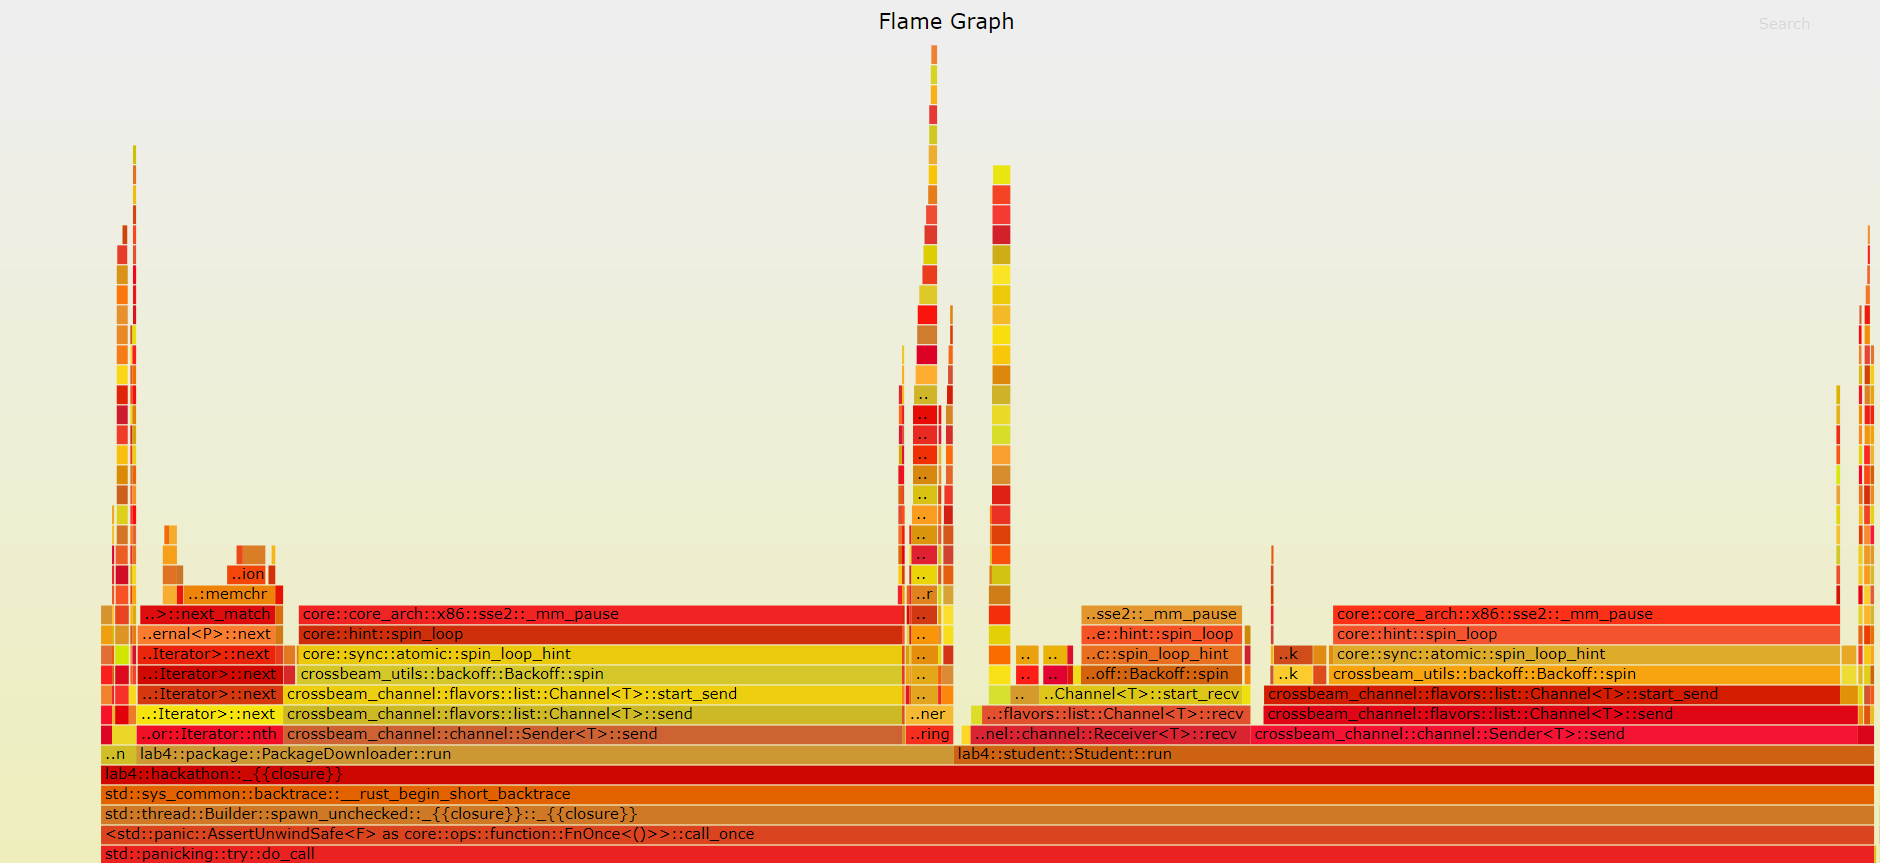
\includegraphics[width=0.8\textwidth]{./flamegraph.png}
	\end{center}
\end{figure}


You probably need to know about how flamegraphs work. To read up on them, see \url{http://www.brendangregg.com/flamegraphs.html}. There are some useful YouTube videos linked there to give you guidance. In particular, the video at \url{https://youtu.be/D53T1Ejig1Q} is useful. If you're in a rush, just watch from the 10 minute mark to about the 16 minute mark.

For your convenience, we've created a Makefile target that runs your program and generates the flamegraph. You'll have to run \texttt{cargo install flamegraph} first. Then, you can create a flamegraph by typing ``make''. This will generate an SVG (Scalable Vector Graphics) file called ``flamegraph.svg''  containing the graph, which can be viewed in any graphical viewing program or in your preferred web browser. We believe that you can create flamegraphs on any of the eceubuntu and ecetesla machines.

\paragraph{Tip.} Want to view SVGs in VS Code? I hear that \texttt{cssho.vscode-svgviewer} is helpful.

In your commit log message, explain how you used your profiling data to decide what to change. Be sure to include the flamegraph for the final version of the program (if not standard flamegraph generation, say how you generated it) and provide some explanation to the reader as to how you used the flamegraph to improve the starter code. Also let us know which machine you measured your results on (it should be one of the ECE machines so that we can reproduce it). (Hint: ecetesla2 doesn't have many threads available!)


\paragraph {Rules/Restrictions.} To prevent trivializing the problem, and to make it possible for us to compare your code against the starter code, here is a list of rules:

\begin{itemize}
	\item You may change how threads communicate.
	\item You may change (or remove) output of intermediate checksums, but the checksums printed out at the end of execution must be identical to the ones generated by the starter code.
        \item You can move IO into main.
	\item You may not change the numbers of student, idea, and package downloader threads (but you can add helper threads).
        \item You can change the provided structs and add, modify, or remove members and their visibility. You can change method signatures as well, e.g. by adding more parameters.
	\item The arguments of the program must still be respected (so you can't change the the number of students/ideas/packages managed by each thread), and you must read the data at runtime.
        \item You can change the lock structure of the program. But don't, for instance, create a single thread to handle checksum updates. Checksum updates stand in for download time.
	\item Must not introduce bugs (memory leaks, deadlocks, etc.). 
	\item Must not trivialize the threads e.g. moving everything to 1 thread to eliminate synchronization. You may rewrite how the threads communicate (different mutex/constructs usage, for example).
	\item All publicly observable final behaviour/output for each thread must be preserved.  You may change intermediate prints (I/O) but not final ones. For example, IdeaGenerator must add \texttt{NewIdea} Events to the queue. It must also be responsible for inserting the poison pills (\texttt{OutOfIdeas}) for the Student threads.
	\item Any threads you create may only be terminated with the \texttt{OutOfIdeas} event (no passing "expected number of ideas").
	\item You must not hardcode any values that are read from files. We will be testing with different files of various sizes.
        \item You can and we encourage you to use any crates that don't trivialize the problem. For instance, you can use \texttt{lazy\_static} and \texttt{once\_cell}. You can use Rayon, though you aren't required to, and it makes the flamegraph harder to read.
        \item You can change the makefile, e.g. to add new targets or change the build flags.
	\item No other changes that trivialize the simulation or execution (e.g. deleting functionality that consumes CPU time). 
\end{itemize}

\section*{Rubric}
We're continuing to require a commit log message instead of a report. Commit messages should still argue for why your change should be merged (including the flamegraph) but imply less boilerplate.

\paragraph{Implementation (35 marks)} Your code must preserve the original behaviour and cannot violate any of the rules specified above. You should make changes, and the changes you make should be supported by a profiling tool of some sort---they can't just be random changes.

\paragraph{Commit Log (15 marks)} 12 marks for explaining the changes that you've made, including your expected speedup results, final flamegraph, and some explanation for the reader. 3 marks for clarity of exposition. 

\paragraph{Performance (50 marks)} For this lab, we are finally measuring performance (with hyperfine). Your code must run faster than the starter code. The faster, the better. Marking guidelines:

\begin{center}
\begin{tabular}{r|r}
\textbf{Speedup ($\times$)} & \textbf(\% of marks for performance)\\ \hline
$\geq 13.5$ & 100\\
$[12, 13.5)$ & 90\\
$[11, 12)$ & 80\\
$[10, 11)$ & 70\\
$[9, 10)$ & 60\\
$[8, 9)$ & 50\\
$[7, 8)$ & 40 \\
$[6, 7)$ & 30\\
$[5, 6)$ & 20\\
$[4, 5)$ & 10\\
$< 4$ & 0
\end{tabular}
\end{center}

We are going to try to run your code on unloaded systems, but if the TA says that they get a different time than you do,
please contact the TA.

\subsection*{What goes in a commit log}
Here's a suggested structure for your commit log message justifying the pull request.
\begin{itemize}
\item Pull Request title explaining the change (less than 80 characters)
\item Summary (about 1 paragraph): brief, high-level description of the work done.
\item Tech details (3--5 paragraphs): anything interesting or noteworthy for the reviewer about how the work is done. 
\item Something about how you tested this code for correctness and know it works (about 1 paragraph)
\item Something about how you tested this code for performance and know it is faster (about 3 paragraphs, referring to the flamegraph as appropriate).
\end{itemize}
Write your message in the file {\tt commit-log/message.md} and commit the final generated flamegraph as the file {\tt commit-log/flamegraph.svg}. Don't forget to {\tt git add commit-log/flamegraph.svg}.

\section*{Clarifications}

\paragraph{Helgrind complains, even on the unmodified code.} Good that you're running Helgrind. Yep, you're not required to fix this.

\paragraph{Which times do you care about?} Hyperfine mean time, taking range and deviations into account.

\paragraph{Is a shared memory queue OK instead of crossbeam?} Yes.

\paragraph{I don't know, man. [unknown] is 50\% of my flamegraph.} Set \texttt{num\_pkgs} to something big, like 100,000.

\paragraph{Just one commit message?} If you want, you can cast your changes as multiple unrelated changes, but you can also 
present them as a single change. Probably easier for the TAs as a single change.

\paragraph{I don't like Events.} You can restructure the program to get rid of the \texttt{Event} type if you feel that is
appropriate, e.g. you want to change the channel structure. (I'm not sure this helps!)

\paragraph{5 isn't enough: I want to write more than 5 paragraphs in the commit log.} Yeah, just don't go overboard, but do
what makes sense.

\paragraph{I don't like 0s.} We aren't going to test your program with any arguments set to 0.

\paragraph{Oh Nondeterminism! no!} You may assume that the number of students $>=$ number of idea generators.
It should be determinstic then. Also, you can assume number of ideas $>$ number of idea generators.

\paragraph{A Blooper to Avoid.} Be sure to use \texttt{hyperfine -i "target/release/lab4"} and not 
\texttt{hyperfine -i "cargo run --release"}.

\paragraph{I don't like doing unnecessary work.} Me neither. But please don't remove calls to \texttt{hex::decode} and \texttt{hex::encode} in \texttt{Checksum::update}. They represent download time.

\paragraph{How many packages?} This is set using a command-line option.

\end{document}
